\documentclass[11pt,a4paper]{article}
\usepackage[a4paper,margin=24mm]{geometry}
\usepackage[T1]{fontenc}
\usepackage[utf8]{inputenc}
\usepackage{lmodern}
\usepackage{amsmath,amssymb,amsthm}
\usepackage{graphicx}
\usepackage{booktabs,array,tabularx,multirow}
\usepackage[font=small,labelfont=bf]{caption}
\usepackage{enumitem}
\usepackage{microtype}
\usepackage{xcolor}
\definecolor{linkblue}{rgb}{0,0.15,0.5}
\usepackage[colorlinks=true,linkcolor=linkblue,citecolor=linkblue,urlcolor=linkblue]{hyperref}
\usepackage{url}
\graphicspath{{./}{figs/}{paper04_minimax_dual_certificates_v20_src/figs/}}
\theoremstyle{plain}
\newtheorem{theorem}{Theorem}[section]
\newtheorem{proposition}[theorem]{Proposition}
\newtheorem{lemma}[theorem]{Lemma}
\newtheorem{corollary}[theorem]{Corollary}
\theoremstyle{definition}
\newtheorem{definition}[theorem]{Definition}
\newtheorem{example}[theorem]{Example}
\newtheorem{openproblem}[theorem]{Open problem}
\theoremstyle{remark}
\newtheorem{remark}[theorem]{Remark}
\newcommand{\R}{\mathbb{R}}
\newcommand{\Qr}{\mathbb{Q}}
\newcommand{\E}{\mathbb{E}}
\newcommand{\Prob}{\mathbb{P}}
\newcommand{\calA}{\mathcal{A}}
\newcommand{\calK}{\mathcal{K}}
\newcommand{\calM}{\mathcal{M}}
\newcommand{\calP}{\mathcal{P}}
\newcommand{\calR}{\mathcal{R}}
\newcommand{\calS}{\mathcal{S}}
\newcommand{\calT}{\mathcal{T}}
\newcommand{\calU}{\mathcal{U}}
\newcommand{\conv}{\operatorname{conv}}
\newcommand{\aff}{\operatorname{aff}}
\newcommand{\rank}{\operatorname{rank}}
\newcommand{\supp}{\operatorname{supp}}
\newcommand{\capi}[1]{\operatorname{cap}_{#1}}
\newcommand{\ind}[1]{\mathbf{1}[#1]}
\newcommand{\tfr}[2]{\tfrac{#1}{#2}}
\newcommand{\dd}{\,\mathrm{d}}
\setlength{\parskip}{2pt}
\emergencystretch=2em
\allowdisplaybreaks

\begin{document}

\title{\textbf{Minimax dual certificates for the common-action obstruction:\\ sparsity, polyhedral recovery, a benchmark law,\\ and the finite review envelope}}
\author{Amin Abaee\\[0.3em]
{\small Independent Researcher}\\[0.2em]
{\small ORCID: \href{https://orcid.org/0000-0002-0019-1842}{0000-0002-0019-1842}\quad
\href{mailto:amin_abaee@ut.ac.ir}{amin\_abaee@ut.ac.ir}}}
\date{October 15, 2026}
\maketitle

\begin{abstract}
\noindent
When a controller must choose one action for every state that its observation cannot distinguish, viability can fail although every state is individually controllable: no action is safe for the whole information atom. This paper gives that \emph{common-action obstruction} a complete dual theory. For control-affine plants with a compact convex action set $U\subset\R^k$ the first-order safe-action constraints of an information atom form a bundle of affine rows, and the obstruction is equivalent---by Sion's theorem---to the existence of a probability measure on the bundle under which the pooled row is strictly negative everywhere on $U$. The measure is a portable certificate: it is checked by one support-function evaluation, it is sound for arbitrary (also non-convex or finite) action sets, and it characterises the convexified obstruction exactly, the parity instance showing that the gap between $U$ and $\conv U$ is real. Helly's theorem bounds the support of a certificate by $\min(\dim\aff U,\rank)+1$ atoms, and a family of plants shows the bound is attained for every $k$; a random study locates typical certificates well below it. For polyhedral $U$ the measure certificate is a Farkas pair whose facet multipliers identify which institutional constraint carries the obstruction. The theory is exercised on a two-stock benchmark with a demand floor $D$: the fibre margin is $\varepsilon^\ast(Y)=(27-5Y)/50$ with the unique certificate $(\tfr12,\tfr12)$, and the critical aggregate stock obeys the piecewise law $Y^\ast(D)=\min(\tfr{77}{5}-5D,\tfr{69}{5})$, whose two branches are a physical and an epistemic--institutional obstruction. The static tests induce a taxonomy of obstructions (physical, epistemic, institutional) with overlapping membership, illustrated on a finite two-patch codex. The dynamic layer is built on finite review trees with action-dependent observation cells: the node recursion equals the supremum over adapted policy trees, committed prefixes inherit node values, posterior-only evaluation is shown not to be an envelope, and the robust value over a class of couplings obeys a certified weak duality whose worst coupling can be interior. On a two-window instance the envelope, the open-loop value and both robust values are tabulated against the initial distance; at distance $4$ every one of the $171$ adapted trees is defeated with probability at least $\tfr38$. An integrated certificate for finite-horizon trajectories with adapted controls reproduces the review threshold $\tau^\ast=\tfr{7}{50}$ of a companion instance. Every number is regenerated by an exact rational script ($66$ checks); the soundness direction, the parity gap and the benchmark algebra are machine-checked in Lean~4.
\end{abstract}

\medskip
\noindent\textbf{Keywords:} viability theory; partial observation; minimax duality; Sion's theorem; Helly's theorem; Farkas certificates; robust control; information design; exact rational verification

\medskip
\noindent\textbf{MSC 2020:} 93B03, 49N30, 90C46, 91A05, 93E20, 52A35
\section{Introduction}\label{sec:intro}

A viability kernel answers the question whether a constrained system can be kept inside its constraints forever \cite{Aubin1991,Aubin2011,Blanchini1999}. Under full state observation the answer is local: the state is viable at first order when some admissible action points the drift inside the constraint set, and Nagumo's condition makes this exact for a large class of sets \cite{Nagumo1942}. Under partial observation the controller does not know the state; it knows an \emph{information atom}, the set $B$ of states compatible with what has been observed, and it must choose one action for all of them. Viability can then fail although every state in $B$ is individually controllable: the safe-action sets of the members of $B$ are non-empty but their intersection is empty. We call this the \emph{common-action obstruction}. It is the mechanism behind the delayed-observation thresholds, the shared-authority ladders and the aggregate-observation failures studied in the companion papers \cite{Abaee2026calc,Abaee2026cert,Abaee2026prob}, and it is the first-order shadow of the output-feedback viability problem.

The question of this paper is how to \emph{certify} such an obstruction: how to produce an object that proves, portably and checkably, that no common action exists. A direct proof enumerates the action set; a certificate should be small, verifiable by a single inequality, and informative about where the obstruction comes from. For control-affine plants with a compact convex action set the answer is a probability measure on the active constraints of the atom. Averaged under the measure, the constraints collapse to a single affine row, and the obstruction is exactly the statement that this row is negative throughout the action set. The equivalence is Sion's minimax theorem in the zero-sum game between the controller, who picks the common action, and an adversary, who picks the state, the constraint and the disturbance. The dual object is a measure because the adversary mixes.

\paragraph{Contributions.} The paper develops this idea into a complete static theory, a taxonomy, a benchmark law and a dynamic layer.
\begin{enumerate}[leftmargin=1.6em,itemsep=1pt]
\item \emph{Static theory} (Section~\ref{sec:static}). Theorem~\ref{thm:dual} states the duality with its exactness: an information atom is obstructed if and only if a measure certificate exists, and the certificate margin equals the negative of the lower value of the game. Remark~\ref{rem:isaacs} identifies the measure dual with the lower value and separates it from the upper value, which is the full-information quantity. Theorem~\ref{thm:helly} bounds the support of a certificate by $\min(\dim\aff U,\rank)+1$ atoms through Helly's theorem---not $k+2$ as Carath\'eodory alone would give---and exhibits, for every $k$, a plant on which the bound is attained. Proposition~\ref{prop:nonconvex} settles the non-convex case: soundness is unconditional, and a certificate exists exactly when the convexified atom is obstructed, so the gap between $U$ and $\conv U$ is the only source of incompleteness. Theorem~\ref{thm:polyhedral} recovers the Farkas form for polyhedral $U$ and shows that the facet multipliers locate the obstruction on specific constraints of the action set.
\item \emph{Taxonomy} (Section~\ref{sec:taxonomy}). Three tests---physical, epistemic, institutional---are defined on the safe-action sets of an atom (Proposition~\ref{prop:taxonomy}). They are tests, not a partition: the institutional test is relative to a reference action set and overlaps with either of the other two. The certificate's support and its facet multipliers read the tests off.
\item \emph{Benchmark law} (Section~\ref{sec:benchmark}). On a two-stock harvesting model with an aggregate observation and a demand floor $D$, Proposition~\ref{prop:benchmark} gives the fibre margin $\varepsilon^\ast(Y)=(27-5Y)/50$, the unique certificate $(\tfr12,\tfr12)$ and its Farkas pair, and Proposition~\ref{prop:floor} the piecewise critical law $Y^\ast(D)=\min(\tfr{77}5-5D,\tfr{69}5)$ whose two branches are, respectively, an epistemic--institutional and a physical obstruction. Each unit of demand floor costs five units of aggregate stock.
\item \emph{Dynamic layer} (Section~\ref{sec:dynamic}). Finite review trees with action-dependent observation cells are defined (Definition~\ref{def:tree}); Theorem~\ref{thm:envelope} proves that the node recursion is the supremum over adapted policy trees, with the tower and martingale identities along any fixed tree, and Corollary~\ref{cor:prefix} that committed prefixes inherit node values. Example~\ref{ex:posterior} shows that posterior-only evaluation is not an envelope. Proposition~\ref{prop:robust} states the certified weak duality of the robust value over a class of couplings and its mixed-policy closure; Example~\ref{ex:sweep} tabulates envelope, open-loop and both robust values on a two-window instance, exhibits an \emph{interior} worst coupling and a dynamically certified obstruction. Proposition~\ref{prop:integrated} is the integrated certificate for finite-horizon trajectories with adapted controls; on the three-branch instance of the companion paper \cite{Abaee2026cert} it reproduces the review threshold $\tau^\ast=\tfr7{50}$ in one line.
\item \emph{Verification} (Section~\ref{sec:verification}). Every number, witness and count is regenerated from the definitions by an exact rational script; the soundness direction, the parity gap and the benchmark algebra are checked in Lean~4. A scope box separates what is proved from what is only computed on instances.
\end{enumerate}

\paragraph{What is new relative to the viability and robust-optimisation literature.} Output-feedback viability has sufficient conditions through set-valued observers and guaranteed viability kernels \cite{Aubin2011,Cardaliaguet2007}; the present dual gives a necessary-and-sufficient first-order criterion with a certificate. The measure certificate is the semi-infinite programming dual \cite{HettichKortanek1993,AndersonNash1987} specialised to affine rows; its Helly-type sparsity is the deterministic counterpart of the support-constraint count of the scenario approach \cite{CalafioreCampi2006,CampiGaratti2008}, where $k+1$ also appears. The dynamic envelope is the finite-horizon dynamic programme of a partially observed problem \cite{Astrom1965,BertsekasShreve1978} written on review trees, which is what makes the tree-supremum identity, the committed-prefix corollary and the posterior-only counterexample elementary; the robust value over couplings is a static-information design problem in the sense of Bergemann and Morris \cite{BergemannMorris2019} with the worst coupling as the designer. The adjustability question of two-stage robust optimisation \cite{WeiZhang2024}, when adaptivity adds value, is the open-loop gap of Section~\ref{sec:dynamic}.

\paragraph{Reading guide.} Section~\ref{sec:setting} fixes the plant, the information atoms and the row abstraction. Sections~\ref{sec:static}--\ref{sec:dynamic} contain the results; proofs that are short are given in place, the longer ones in the supplementary material, which also contains the complete instance records, the random study, the Lean scope list and a symbol table with sign conventions. Section~\ref{sec:verification} describes the verification record, Section~\ref{sec:related} places the results and lists open problems.
\section{Setting: plants, information atoms and the row bundle}\label{sec:setting}

\paragraph{Plant and constraints.} The state $x\in\R^n$ obeys the control-affine dynamics
\begin{equation}\label{eq:plant}
\dot x=f(x,u,d)=f_0(x,d)+G(x)\,u,\qquad u\in U\subset\R^k,\quad d\in D\subset\R^m,
\end{equation}
with $U$ compact and convex, $D$ compact, $f_0$ continuous and $G$ continuous. The constraint set is $\calS=\{x:\ q_j(x)\ge0,\ j\in J\}$ with finitely many $C^1$ functions $q_j$. For $x\in\calS$ let $J(x)=\{j:\ q_j(x)=0\}$ be the active index set. The \emph{first-order safe-action set} at $x$ is
\begin{equation}\label{eq:R}
\begin{gathered}
\calR(x)=\bigl\{u\in U:\ \psi_{x,j,d}(u)\ge0\ \text{ for all } j\in J(x),\ d\in D\bigr\},\\
\psi_{x,j,d}(u)=\nabla q_j(x)^{\!\top}f_0(x,d)+\nabla q_j(x)^{\!\top}G(x)\,u .
\end{gathered}
\end{equation}
Each $\psi_{x,j,d}$ is affine in $u$: $\psi_{x,j,d}(u)=c_a+v_a^{\top}u$ with $a=(x,j,d)$, $c_a=\nabla q_j(x)^\top f_0(x,d)$ and $v_a=G(x)^\top\nabla q_j(x)$. The set $\calR(x)$ collects the actions whose worst-case drift is sub-tangential to every active constraint. If the active gradients satisfy a constraint qualification at $x$ (for instance linear independence, or $\calS$ polyhedral near $x$), the contingent cone of $\calS$ at $x$ is the linearised cone, and $\calR(x)\neq\emptyset$ is necessary for $x$ to belong to the viability kernel of \eqref{eq:plant} \cite{Aubin1991,Nagumo1942}; without a qualification it remains a necessary condition for the linearised problem and we use it as such. When $\psi_{x,j,d}\equiv0$ on $U$ for an active constraint (a tangential drift of second order) the first-order test is silent, and higher-order conditions are needed; such atoms are outside the scope of the first-order theory and are flagged, not classified, by the tests below.

\paragraph{Information atoms.} An observation does not reveal $x$ but an \emph{atom} $B\subset\calS$, the set of states compatible with it. The controller chooses one $u$ for the whole atom. The \emph{common safe-action set} and the \emph{active bundle} of $B$ are
\begin{equation}\label{eq:common}
\calR(B)=\bigcap_{x\in B}\calR(x),\qquad \calK(B)=\{(x,j,d):\ x\in B,\ j\in J(x),\ d\in D\}.
\end{equation}
Throughout, $B$ is a compact set on which the active index set is locally constant on finitely many pieces, so that $\calK(B)$ is a compact index set on which $a\mapsto(c_a,v_a)$ is continuous (in the examples $B$ is finite or a segment). We say that $B$ is \emph{obstructed} when $\calR(B)=\emptyset$.

\paragraph{The row abstraction.} All statements of Sections~\ref{sec:static}--\ref{sec:taxonomy} concern only the family of affine rows $\{\psi_a(u)=c_a+v_a^\top u:\ a\in\calA\}$ indexed by a compact set $\calA$ (in the application $\calA=\calK(B)$), and the action set $U$. We write
\begin{equation}\label{eq:values}
V^-=\max_{u\in U}\ \min_{a\in\calA}\psi_a(u),\qquad V^+=\min_{a\in\calA}\ \max_{u\in U}\psi_a(u),\qquad
\Phi(u,\mu)=\int_{\calA}\psi_a(u)\dd\mu(a)
\end{equation}
for the lower and upper values of the zero-sum game in which the controller picks $u$ and the adversary picks the row, and for the mixed-adversary payoff with $\mu\in\calP(\calA)$, the probability measures on $\calA$. The common safe-action set is $\{u\in U:\ \min_a\psi_a(u)\ge0\}$, so $B$ is obstructed exactly when $V^-<0$; the maxima and minima in \eqref{eq:values} are attained by compactness and continuity. The \emph{support function} of $U$ is $h_U(g)=\max_{u\in U}g^\top u$.

\begin{definition}[measure certificate]\label{def:certificate}
A probability measure $\mu\in\calP(\calA)$ is a \emph{certificate} for the row family if
\begin{equation}\label{eq:cert}
\varepsilon(\mu)\;:=\;-\max_{u\in U}\Phi(u,\mu)\;=\;-\Bigl(\int c_a\dd\mu+h_U\Bigl(\int v_a\dd\mu\Bigr)\Bigr)\;>\;0 ;
\end{equation}
$\varepsilon(\mu)$ is its \emph{margin}. Since $\Phi(\cdot,\mu)$ is affine, the maximum in \eqref{eq:cert} is a single support-function evaluation at the pooled coefficient vector $\bar v=\int v_a\dd\mu$: checking a certificate costs one evaluation of $h_U$, which for polyhedral $U$ is a maximum over vertices and for an ellipsoid is a norm.
\end{definition}

Soundness of a certificate is one line and holds for \emph{every} $U$, convex or not: if $u\in\calR(B)$ then $\psi_a(u)\ge0$ for all $a$, hence $\Phi(u,\mu)\ge0$, contradicting $\varepsilon(\mu)>0$. This is the direction formalised in Lean (Section~\ref{sec:verification}). The content of the theory is the converse, the size of certificates, and what they say about the obstruction.
\section{The static theory}\label{sec:static}

\subsection{Duality and exactness}

\begin{theorem}[measure dual of the common-action obstruction]\label{thm:dual}
Let $U\subset\R^k$ be compact and convex and let $\{\psi_a=c_a+v_a^\top u:\ a\in\calA\}$ be a family of affine rows indexed by a compact set $\calA$ with $a\mapsto(c_a,v_a)$ continuous. Then
\begin{equation}\label{eq:sion}
\max_{u\in U}\ \min_{a\in\calA}\psi_a(u)\;=\;\min_{\mu\in\calP(\calA)}\ \max_{u\in U}\ \Phi(u,\mu),
\end{equation}
both extrema being attained. Consequently the following are equivalent: (i) the common safe-action set $\{u\in U:\min_a\psi_a(u)\ge0\}$ is empty; (ii) $V^-<0$; (iii) a certificate exists. When they hold, the best margin is $\max_\mu\varepsilon(\mu)=-V^->0$, and every measure $\mu^\ast$ attaining the right-hand side of \eqref{eq:sion} is a certificate of maximal margin.
\end{theorem}

\begin{proof}
$\Phi$ is bilinear in $(u,\mu)$, continuous on $U\times\calP(\calA)$ when $\calP(\calA)$ carries the weak$^\ast$ topology (by continuity of $a\mapsto(c_a,v_a)$), $U$ is compact convex and $\calP(\calA)$ is compact convex. Sion's theorem \cite{Sion1958} gives $\max_u\min_\mu\Phi=\min_\mu\max_u\Phi$. For fixed $u$ the minimum of $\mu\mapsto\int\psi_a(u)\dd\mu$ over $\calP(\calA)$ is attained at a Dirac mass and equals $\min_a\psi_a(u)$; this yields \eqref{eq:sion}. The equivalences follow: (i)$\Leftrightarrow$(ii) because the minimum over $a$ is attained; (ii)$\Leftrightarrow$(iii) because the right-hand side of \eqref{eq:sion} is $-\max_\mu\varepsilon(\mu)$.
\end{proof}

\begin{remark}[lower value, upper value and what the measure buys]\label{rem:isaacs}
In the terminology of games \cite{Isaacs1965,BasarOlsder1999}, $V^-$ is the lower value (the controller commits to a common action, the adversary answers with the worst row) and $V^+$ is the upper value (the row is announced first, so the controller may answer with an action adapted to it---the full-information situation). Always $V^-\le V^+$. Theorem~\ref{thm:dual} says that the \emph{mixed-adversary} value equals the lower value: letting the adversary randomise over rows costs the controller nothing beyond what the common action already costs, and the mixing measure is the certificate. The two values separate exactly the information effect. On $U=[0,1]$ with rows $1-2u$ and $2u-1$ one has $V^-=0$ (at $u=\tfr12$) and $V^+=1$: with full information each row is comfortably satisfied, under the common action the atom is viable only at the boundary. The conditions $V^+<0$ and $V^-<0$ delimit the two faces of the taxonomy of Section~\ref{sec:taxonomy}: $V^+<0$ means that one row alone is infeasible, which forces a physical obstruction; $V^+\ge0>V^-$ is the band in which every row is individually satisfiable.
\end{remark}

Figure~\ref{fig:dual} shows the geometry on one-dimensional instances. On the \emph{two-floor instance} $U=[0,1]$ with rows $\psi_1(u)=\tfr25-u$ and $\psi_2(u)=u-\tfr35$ (two states with floors at $\tfr25$ and $\tfr35$ pulling in opposite directions) the lower envelope peaks at $V^-=-\tfr1{10}$, attained at $u=\tfr12$, and $\mu^\ast=(\tfr12,\tfr12)$ pools the rows to the constant $-\tfr1{10}$: a certificate of margin $\tfr1{10}$. Moving the second floor to $\tfr15$ gives $V^-=+\tfr1{10}$ at $u=\tfr3{10}$, and every pooled row is positive somewhere: no certificate exists, as the theorem predicts.

\begin{figure}[t]
\centering
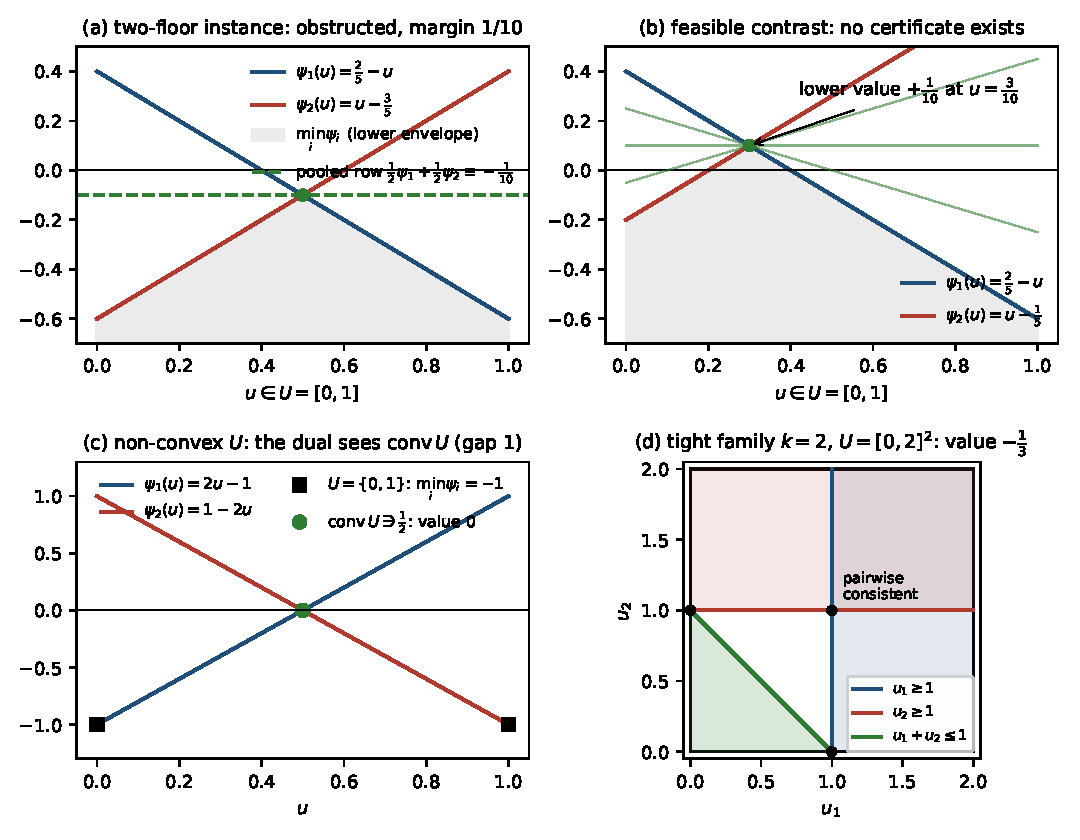
\includegraphics[width=\textwidth]{fig1_dual_geometry.pdf}
\caption{The measure dual on one- and two-dimensional instances (Theorem~\ref{thm:dual}, Theorem~\ref{thm:helly}, Proposition~\ref{prop:nonconvex}). (a) Two-floor instance: the lower envelope peaks at $-\tfr1{10}$ and the equal-weight pooled row is the constant $-\tfr1{10}$. (b) Feasible contrast: the envelope peaks at $+\tfr1{10}$ and every pooled row (thin lines) is positive somewhere. (c) Parity instance on the non-convex $U=\{0,1\}$: the value over $U$ is $-1$, the value over $\conv U$ is $0$, so no certificate exists although the atom is obstructed. (d) The tight family for $k=2$: three half-planes, pairwise consistent on $U=[0,2]^2$, with empty triple intersection; the lower value is $-\tfr13$ and the uniform measure is the unique optimal certificate.}
\label{fig:dual}
\end{figure}

\subsection{Sparsity: Helly, not Carath\'eodory}

\begin{theorem}[support of a certificate]\label{thm:helly}
Under the hypotheses of Theorem~\ref{thm:dual}, suppose the row family is obstructed. Let $d=\dim\aff U$ and $r=\rank\{v_a:\ a\in\calA\}$. Then
\begin{enumerate}[leftmargin=1.6em,itemsep=1pt]
\item[(i)] there is a certificate supported on at most $s=\min(d,r)+1$ rows; moreover some $s$ rows are already jointly infeasible on $U$;
\item[(ii)] the bound is attained for every $k$: on $U=[0,k]^k$ the $k+1$ rows $u_i-1\ge0$ $(i=1,\dots,k)$ and $(k-1)-\sum_iu_i\ge0$ are infeasible, every $k$ of them are feasible, the lower value is $-\tfr1{k+1}$, and the uniform measure is a certificate of margin $\tfr1{k+1}$. These rows are the active bundle at the origin of the plant $\dot x_i=-1+u_i$ $(i\le k)$, $\dot x_{k+1}=(k-1)-\sum_iu_i$ with constraints $x_j\ge0$ and no disturbance.
\end{enumerate}
\end{theorem}

\begin{proof}
(i) Let $C_a=\{u\in U:\ \psi_a(u)\ge0\}$, a compact convex subset of $U$. Obstruction means $\bigcap_aC_a=\emptyset$. If $r<k$, let $P$ be the orthogonal projection onto the span $W$ of the $v_a$; since $\psi_a(u)=c_a+v_a^\top Pu$, the sets $C_a$ are the preimages under $P|_U$ of the compact convex sets $C_a'=\{w\in P(U):\ c_a+v_a^\top w\ge0\}\subset W\cong\R^r$, and $\bigcap_aC_a=\emptyset$ iff $\bigcap_aC_a'=\emptyset$. Helly's theorem for an arbitrary family of compact convex sets in a space of dimension $e$ \cite{Helly1923,Rockafellar1970} states that if every $e+1$ members intersect then the family intersects. Applied in $W$ (dimension $r$) or in $\aff U$ (dimension $d$), it produces $s=\min(d,r)+1$ rows $a_1,\dots,a_s$ with $C_{a_1}\cap\dots\cap C_{a_s}=\emptyset$. Theorem~\ref{thm:dual} applied to the finite family $\{\psi_{a_1},\dots,\psi_{a_s}\}$ gives a certificate supported on these rows; it is a certificate for the whole family because $\Phi(u,\mu)$ only involves the rows in the support. (ii) Removing the sum row, $u=(1,\dots,1)$ is feasible; removing the row $u_i-1\ge0$, the point with $u_i=0$ and $u_j=1$ for $j\ne i$ satisfies $\sum u_j=k-1$. All $k+1$ rows force $\sum_iu_i\ge k>k-1$. At $u=(t,\dots,t)$ the rows equal $t-1$ and $(k-1)-kt$, which coincide at $t=\tfr{k}{k+1}$ with value $-\tfr1{k+1}$; the uniform measure pools the rows to the constant $-\tfr1{k+1}$, so by weak duality (soundness) $V^-=-\tfr1{k+1}$ and the margin $\tfr1{k+1}$ is maximal. The plant statement is the computation $\nabla q_j^\top f=\dot x_j$ at $x=0$, where all $k+1$ constraints are active.
\end{proof}

Carath\'eodory's theorem applied to the pooled row $(\int c\dd\mu,\int v\dd\mu)\in\conv\{(c_a,v_a)\}\subset\R^{k+1}$ would give $k+2$ atoms; the Helly route gives $k+1$, and the refinement by the rank of the drift coefficients is what makes the bound small in applications: in the benchmark of Section~\ref{sec:benchmark} the two coefficient vectors $(-1,0)$ and $(0,-1)$ span $\R^2$ and the certificate has two atoms; in the three-branch instance of Section~\ref{sec:integrated} the three normals span $\R^2$ and the certificate has three atoms, which is $r+1$.

\begin{remark}[typical and worst-case support]\label{rem:random}
The worst case of Theorem~\ref{thm:helly} is attained, but a random study (supplementary S4) shows that it is rare. Drawing rows with integer coefficients in $\{-3,\dots,3\}$ on $U=[-1,1]^k$ and locating, for every infeasible system, the smallest infeasible subfamily by exact enumeration, the size $k+1$ occurred in $54$ of $217$ infeasible systems for $k=1$, in $9$ of $214$ for $k=2$ and in $2$ of $86$ for $k=3$, and not at all in the $65$ infeasible systems drawn for $k=4$, where the largest support found was $4$ (in $5$ systems); always $m=k+3$ rows. With rank-one coefficient vectors in $k=3$ the size never exceeded $2$, as (i) requires. The size of the witness must not be confused with the cost of finding it: locating a minimal infeasible subfamily by enumeration costs $\binom{m}{s}$ feasibility tests, whereas a certificate of maximal margin is one linear programme over all $m$ rows (Remark~\ref{rem:search}).
\end{remark}

\subsection{Non-convex action sets}

\begin{proposition}[soundness is unconditional; exactness is convexification]\label{prop:nonconvex}
Let $U\subset\R^k$ be any compact set and let the row family be as in Theorem~\ref{thm:dual}. Then
\begin{enumerate}[leftmargin=1.6em,itemsep=1pt]
\item[(i)] every certificate (Definition~\ref{def:certificate} with the maximum over $U$) proves that no common safe action exists in $U$;
\item[(ii)] a certificate exists if and only if the convexified family---the same rows on $\conv U$---is obstructed; the margin computed over $U$ and over $\conv U$ coincide;
\item[(iii)] the gap is real: on $U=\{0,1\}$ with rows $2u-1$ and $1-2u$ (the \emph{parity instance}) the value over $U$ is $-1$, so the atom is obstructed, while the value over $\conv U=[0,1]$ is $0$ and no certificate exists.
\end{enumerate}
\end{proposition}

\begin{proof}
(i) is the one-line soundness argument after Definition~\ref{def:certificate}. (ii) The maximum of the affine function $\Phi(\cdot,\mu)$ over $U$ equals its maximum over $\conv U$; hence $\mu$ is a certificate for $U$ iff it is one for $\conv U$, and Theorem~\ref{thm:dual} applies to $\conv U$. (iii) On $U$ both actions give $\min_a\psi_a=-1$; on $\conv U$ the point $\tfr12$ gives $0$, so $V^-_{\conv U}=0$ and by (ii) and Theorem~\ref{thm:dual} no certificate exists.
\end{proof}

The proposition replaces the informal statement that non-convex obstructions are ``located at the boundary'': the correct statement is that the dual certifies exactly the convexified obstruction. The residual obstruction---an atom obstructed on $U$ but not on $\conv U$---is a statement about the admissibility of mixtures. If relaxed (chattering) controls are admissible, the convex hull is the right action set and the residual disappears; if actions are indivisible, as in the finite codex of Section~\ref{sec:taxonomy}, the obstruction must be certified combinatorially, which for finite $U$ is a finite check and for finite $U$ in a finite horizon is what the review trees of Section~\ref{sec:dynamic} do exactly. The Lean module proves both halves of (iii) (Section~\ref{sec:verification}).

\subsection{Polyhedral action sets: the Farkas form and its facet multipliers}

\begin{theorem}[polyhedral recovery]\label{thm:polyhedral}
Let $U=\{u\in\R^k:\ Au\le b\}$ be a non-empty polytope ($A\in\R^{p\times k}$) and let $\calA$ be finite with rows $\psi_a=c_a+v_a^\top u$. The following are equivalent: (i) $\calR=\{u\in U:\psi_a(u)\ge0\ \forall a\}=\emptyset$; (ii) there exist $\lambda\in\Delta(\calA)$ (the simplex) and $\nu\in\R^p_{\ge0}$ with
\begin{equation}\label{eq:farkas}
\sum_a\lambda_av_a=A^\top\nu,\qquad \sum_a\lambda_ac_a+b^\top\nu<0 .
\end{equation}
For such a pair, $\lambda$ is a certificate in the sense of Definition~\ref{def:certificate} with margin $\varepsilon(\lambda)\ge-(\sum_a\lambda_ac_a+b^\top\nu)$, with equality when $\nu$ is an optimal solution of the linear programme $\min\{b^\top\nu:\ A^\top\nu=\sum_a\lambda_av_a,\ \nu\ge0\}$, whose value is $h_U(\sum_a\lambda_av_a)$. Conversely every certificate $\lambda$ extends to a pair \eqref{eq:farkas} by taking $\nu$ optimal in that programme.
\end{theorem}

\begin{proof}
$\calR$ is the solution set of the linear system $-v_a^\top u\le c_a$ $(a\in\calA)$, $Au\le b$. By Farkas' lemma \cite{Farkas1902,Chvatal1983} it is empty iff some non-negative combination $(\lambda,\nu)$ of the rows yields the contradiction $0<0$, i.e. $-\sum_a\lambda_av_a+A^\top\nu=0$ and $\sum_a\lambda_ac_a+b^\top\nu<0$. If $\lambda=0$ then $A^\top\nu=0$ and $b^\top\nu<0$, which by Farkas again means $U=\emptyset$; so $\lambda\neq0$ and may be normalised to the simplex. By linear programming duality $h_U(g)=\max\{g^\top u: Au\le b\}=\min\{b^\top\nu: A^\top\nu=g,\ \nu\ge0\}$, which gives the margin identity and the converse.
\end{proof}

The facet multipliers $\nu$ carry information that the measure alone does not: they say which constraints \emph{of the action set} the obstruction is charged to. In the benchmark the only positive multiplier sits on the demand-floor facet, so lifting that facet removes the obstruction (Proposition~\ref{prop:benchmark}(iv)); this is how the institutional test of Section~\ref{sec:taxonomy} is read off a certificate. The Lean lemma \texttt{benchmark\_obstruction} is the instance of \eqref{eq:farkas} with $\lambda=(\tfr12,\tfr12)$ and $\nu=\tfr12$.

\begin{remark}[witness size versus search cost]\label{rem:search}
For finite $\calA$ with $m$ rows, both $V^-$ and a certificate of maximal margin are obtained from one linear programme in $k+1$ variables and $m+p$ constraints, in polynomial time; the exact rational optimum is a vertex and therefore rational when the data are. The role of the certificate is not to speed up the primal test but to make its outcome \emph{portable}: the verifier of the certificate needs only the $s\le\min(d,r)+1$ rows in its support and one evaluation of $h_U$, does not need to trust the solver, and can be a proof assistant. The companion paper \cite{Abaee2026cert} uses exactly this division of labour for the finite-horizon programmes of which Theorem~\ref{thm:dual} is the one-step kernel.
\end{remark}
\section{Three tests on an obstructed atom}\label{sec:taxonomy}

The static theory separates two questions that are often conflated: whether an atom is obstructed because some state in it cannot be saved at all, or because the states can be saved only by different actions. A third question is whether the obstruction is an artefact of the action set the controller has been given. The following tests make the three questions precise for an arbitrary action set $U$ (convex or finite); the certificate reads them off when $U$ is convex.

\begin{proposition}[physical, epistemic and institutional tests]\label{prop:taxonomy}
Let $B$ be an atom with safe-action sets $\calR_U(x)$, $x\in B$, and let $U'\supseteq U$ be a reference action set. Define
\begin{align*}
\text{(P) physical:}\quad&\exists\,x\in B:\ \calR_U(x)=\emptyset;\\
\text{(E) epistemic:}\quad&\calR_U(x)\neq\emptyset\ \ \forall x\in B\quad\text{and}\quad\bigcap_{x\in B}\calR_U(x)=\emptyset;\\
\text{(I) institutional (relative to $U'$):}\quad&\bigcap_{x\in B}\calR_U(x)=\emptyset\quad\text{and}\quad\bigcap_{x\in B}\calR_{U'}(x)\neq\emptyset .
\end{align*}
Then: (i) an obstructed atom satisfies exactly one of (P), (E); (ii) (I) is relative to $U'$ and can hold together with either (P) or (E); (iii) if $U$ is compact convex and the rows satisfy the hypotheses of Theorem~\ref{thm:dual}, then (P) holds iff some certificate is supported on the rows of a single state, and (E) holds iff the atom is obstructed and every certificate charges at least two states; (iv) if $U$ and $U'$ are polytopes, (I) holds iff a pair \eqref{eq:farkas} exists for $U$ and none exists for $U'$; and if some pair for $U$ has $\nu=0$, the obstruction persists for every $U'\supseteq U$ with the same rows, so (I) fails for all reference sets.
\end{proposition}

\begin{proof}
(i) is immediate from the definitions. (ii) Example~\ref{ex:patch} exhibits both combinations. (iii) If $\calR_U(x)=\emptyset$, Theorem~\ref{thm:dual} applied to the atom $\{x\}$ gives a certificate supported on the rows of $x$, which is a certificate for $B$; conversely a certificate supported on the rows of $x$ proves $\calR_U(x)=\emptyset$ by soundness. (iv) is Theorem~\ref{thm:polyhedral} applied to $U$ and $U'$. For the last clause: if $\nu=0$ then $\sum_a\lambda_av_a=0$ and $\sum_a\lambda_ac_a<0$, so $\Phi(\cdot,\lambda)$ is a negative constant on all of $\R^k$ and the certificate is valid for every action set.
\end{proof}

The tests are deliberately \emph{not} a partition. (P) says that better information cannot help at $x$; (E) says that resolving the atom would; (I) says that enlarging the codex would. An obstruction can be epistemic and institutional at once (the benchmark band of Proposition~\ref{prop:floor}), or physical and institutional (a corner whose only escape is a forbidden action). The certificate is the common currency: its support says whether a single state suffices, its facet multipliers say which constraints of $U$ are charged, and a certificate with $\nu=0$ is a proof that no institutional relaxation of $U$ can help.

\begin{example}[a finite two-patch codex]\label{ex:patch}
Two patches hold stocks $x_1,x_2\in\{0,1,2,3\}$; the safe set is $x_1,x_2\ge1$. In each period the manager spares one patch, which regrows by one unit (capped at $3$), while the other regrows by one unit and is harvested by two. The action set is finite, $U=\{\text{spare }1,\text{spare }2\}$, so the measure dual does not apply and the tests are combinatorial. There are $9$ safe states; the viability kernel under both actions has $8$ states, all safe states except $(1,1)$, where neither action is safe: the atom $\{(1,1)\}$ is \emph{physical}. The atom $\{(1,2),(2,1)\}$ is \emph{epistemic}: the safe actions are $\{\text{spare }1\}$ at $(1,2)$ and $\{\text{spare }2\}$ at $(2,1)$, each non-empty, with empty intersection. The \emph{institutional} test relative to the two-action codex: restricting the manager to a single fixed action, whichever one, empties the kernel ($8\to0$), so every atom is institutional relative to the full codex. Under the codex $\{\text{spare }2\}$ the singleton atom $\{(1,2)\}$ is physical (its only admissible action is unsafe) and institutional relative to the full codex (which saves it): both tests hold at once, and the atom $\{(1,1),(2,2)\}$ shows the other overlap pattern, physical under every codex and therefore never institutional. All counts are regenerated by the verification script (checks T1.1--T1.4).
\end{example}
\section{The two-stock benchmark and the demand-floor law}\label{sec:benchmark}

\paragraph{Model.} Two interacting stocks are harvested under an aggregate observation and a demand floor:
\begin{equation}\label{eq:bench}
\dot x_i=r_ix_i\Bigl(1-\frac{x_i}{10}\Bigr)-\frac{x_1x_2}{20}-u_i+d_i,\qquad i=1,2,
\end{equation}
with $r=(1,\tfr45)$, shocks $|d_i|\le\tfr1{10}$, constraints $q_i(x)=x_i-2\ge0$ (conservation floors), and the action set
\begin{equation}\label{eq:benchU}
U_D=\bigl\{u\in[0,2]^2:\ u_1+u_2\ge D\bigr\},\qquad D=2\ \text{unless stated otherwise},
\end{equation}
a polytope whose last facet is the demand floor. The controller observes only the aggregate stock $Y=x_1+x_2$, so its atom on the band $Y\ge4$ is the fibre $B_Y=\{x\in\calS:\ x_1+x_2=Y\}$. Along the fibre the constraint $q_i$ is active only at the corner $x^{(i)}$ where $x_i=2$; interior points of the fibre have no active constraint and contribute no row. The active bundle $\calK(B_Y)$ therefore consists of the rows of the two corners, one per shock value, and the worst shock $d_i=-\tfr1{10}$ gives the binding rows
\begin{equation}\label{eq:caps}
\psi_i(u)=\capi{i}(Y)-u_i,\qquad \capi{1}(Y)=\tfr32-\tfr{Y-2}{10},\qquad \capi{2}(Y)=\tfr{59}{50}-\tfr{Y-2}{10},
\end{equation}
obtained by evaluating \eqref{eq:bench} at $x^{(1)}=(2,Y-2)$ and $x^{(2)}=(Y-2,2)$: $\capi{1}(Y)=1\cdot2\cdot\tfr45-\tfr{2(Y-2)}{20}-\tfr1{10}$ and $\capi{2}(Y)=\tfr45\cdot2\cdot\tfr45-\tfr{2(Y-2)}{20}-\tfr1{10}$. Both caps lie in $[0,2]$ for $Y\in[4,\tfr{69}5]$, so the box facets of $U_D$ are never charged on that band and the only constraint of $U_D$ that can bind is the floor. The fibre is \emph{first-order viable under the aggregate observation} when $\calR(B_Y)=\{u\in U_D:\ u_1\le\capi{1}(Y),\ u_2\le\capi{2}(Y)\}\neq\emptyset$. (The first-order test is necessary for viability; it is not claimed to be sufficient along the whole band.)

\begin{proposition}[fibre margin, certificate and Farkas pair]\label{prop:benchmark}
For $D=2$ and $Y\in[4,\tfr{69}5]$:
\begin{enumerate}[leftmargin=1.6em,itemsep=1pt]
\item[(i)] the lower value of the fibre is $\varepsilon^\ast(Y)=\max_{u\in U_2}\min_i\psi_i(u)=\tfr{27-5Y}{50}$, attained at the $Y$-independent action $u^\ast=(\tfr{29}{25},\tfr{21}{25})$; the fibre is first-order viable iff $Y\le Y^\ast=\tfr{27}5$, equivalently iff its width $Y-4$ is at most $\tfr75$;
\item[(ii)] for every $Y$ the unique measure attaining the dual value is $\mu^\ast=(\tfr12,\tfr12)$ on the two worst-shock corner rows, with margin $-\varepsilon^\ast(Y)$ when $Y>\tfr{27}5$; the four-atom bundle (both shocks) has the same value and its optimal measure charges only the worst-shock atoms;
\item[(iii)] the Farkas pair of Theorem~\ref{thm:polyhedral} is $\lambda=(\tfr12,\tfr12)$, $\nu=\tfr12$ on the demand facet $-u_1-u_2\le-2$ and $\nu=0$ on the box facets: $\sum\lambda_av_a=(-\tfr12,-\tfr12)=\tfr12\,(-1,-1)$ and $\sum\lambda_ac_a+b^\top\nu=\tfr{\capi{1}+\capi{2}}{2}-1=\varepsilon^\ast(Y)$;
\item[(iv)] on the band $Y\in(\tfr{27}5,\tfr{69}5)$ each corner is first-order viable alone ($\capi{i}(Y)\ge0$) and the pair is not: the obstruction is epistemic; it is institutional relative to the box $U_0=[0,2]^2$, on which the fibre is viable with margin $\min_i\capi{i}(Y)>0$.
\end{enumerate}
At $Y=6$: $\capi{1}=\tfr{11}{10}$, $\capi{2}=\tfr{39}{50}$, cap sum $\tfr{47}{25}<2$, margin $-\tfr3{50}$; at $Y=5$ the common action $(\tfr65,\tfr45)$ is safe and the maximiser $(\tfr{29}{25},\tfr{21}{25})$ has margin $\tfr1{25}$; at $Y=4$ the caps are $\tfr{13}{10}$ and $\tfr{49}{50}$ with margin $\tfr7{50}$.
\end{proposition}

\begin{proof}
(i) For $u\in U_2$, $\min_i(\capi{i}-u_i)\le\tfr12\sum_i(\capi{i}-u_i)\le\tfr12(\capi{1}+\capi{2}-2)$, with equality at $u=(\capi{1}-\varepsilon,\capi{2}-\varepsilon)$, $\varepsilon=\tfr12(\capi{1}+\capi{2}-2)$, i.e. at $u^\ast=\tfr12(\capi{1}-\capi{2}+2,\ \capi{2}-\capi{1}+2)=(\tfr{29}{25},\tfr{21}{25})$, which does not depend on $Y$ and lies in $U_2$. Substituting \eqref{eq:caps} gives $\tfr{27-5Y}{50}$, which vanishes at $\tfr{27}5$. (ii) For $\lambda=(\lambda_1,\lambda_2)$ the pooled maximum over $U_2$ is $\lambda_1\capi{1}+\lambda_2\capi{2}-\min_{u\in U_2}(\lambda_1u_1+\lambda_2u_2)=\lambda_1\capi{1}+\lambda_2\capi{2}-2\min(\lambda_1,\lambda_2)$, which on either side of $\lambda_1=\tfr12$ is strictly monotone in $\lambda_1$ because $\capi{1}-\capi{2}+2>0$ and $\capi{2}-\capi{1}+2>0$; the minimum is at $\lambda=(\tfr12,\tfr12)$. The four-atom statement is a direct computation (check B2.3). (iii) is read off \eqref{eq:farkas} with $A$ the facet matrix of $U_2$ and $b$ its right-hand side; the box facets receive multiplier $0$. (iv) $\capi{2}(Y)\ge0$ iff $Y\le\tfr{69}5$ and $\capi{1}\ge\capi{2}$; at corner $i$ alone the action $u=(0,2)$ or $(2,0)$ is admissible and safe. On $U_0$ the common action $u=0$ is safe with margin $\min_i\capi{i}(Y)$.
\end{proof}

\begin{proposition}[demand-floor law]\label{prop:floor}
Let $Y^\ast(D)=\sup\{Y\ge4:\ \calR_{U_D}(B_Y)\neq\emptyset\}$ be the critical aggregate stock under the floor $D\in[0,4]$. Then
\begin{equation}\label{eq:floorlaw}
Y^\ast(D)=\min\Bigl(\tfrac{77}{5}-5D,\ \tfrac{69}{5}\Bigr)\quad\text{for }D\le\tfr{57}{25},\qquad\text{and no fibre } Y\ge4 \text{ is viable for } D>\tfr{57}{25}.
\end{equation}
For $D<\tfr8{25}$ the threshold $\tfr{69}5$ is a physical obstruction (the cap of corner $2$ vanishes); for $D\in(\tfr8{25},\tfr{57}{25}]$ the threshold $\tfr{77}5-5D$ is epistemic and institutional, with slope $-5=-\bigl(2\cdot\tfr1{20}\cdot2\bigr)^{-1}$: each unit of demand floor costs five units of aggregate stock. $D=2$ recovers $Y^\ast=\tfr{27}5$.
\end{proposition}

\begin{proof}
The fibre is viable iff $\capi{i}(Y)\ge0$ for both $i$ and $\capi{1}(Y)+\capi{2}(Y)\ge D$ (the same argument as in Proposition~\ref{prop:benchmark}(i) with $2$ replaced by $D$). The first condition is $Y\le\tfr{69}5$, the second $Y\le\tfr{77}5-5D$ since $\capi{1}+\capi{2}=\tfr{77}{25}-\tfr Y5$. The two lines cross at $D=\tfr8{25}$, and $\tfr{77}5-5D\ge4$ iff $D\le\tfr{57}{25}$. The classification follows from Proposition~\ref{prop:benchmark}(iv) with $2$ replaced by $D$. The script verifies the zero, the sign change on both sides and the regime boundaries on a rational grid of $D$ (checks B4.1--B4.4).
\end{proof}

\begin{figure}[t]
\centering
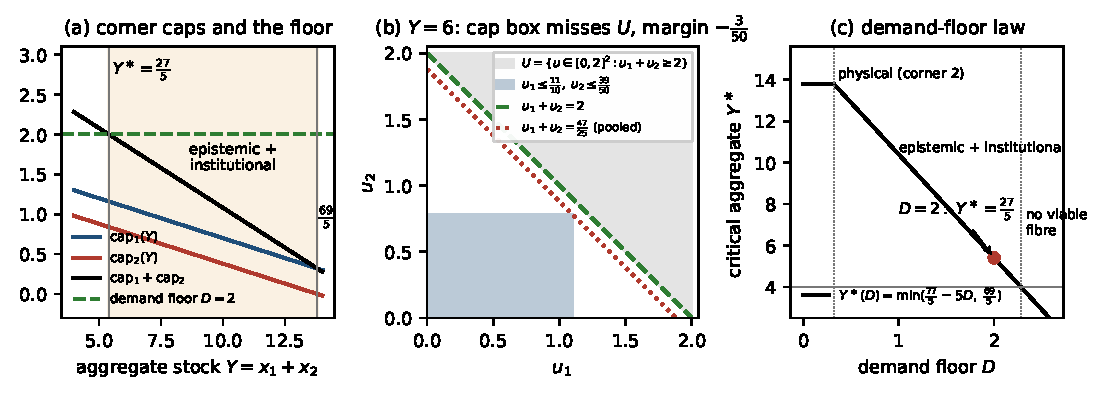
\includegraphics[width=\textwidth]{fig2_benchmark.pdf}
\caption{The two-stock benchmark (Propositions~\ref{prop:benchmark} and~\ref{prop:floor}). (a) Corner caps, their sum and the demand floor $D=2$ as functions of the aggregate stock; the shaded band $(\tfr{27}5,\tfr{69}5)$ is the epistemic--institutional obstruction. (b) The control set $U_2$ and the cap box at $Y=6$: the box $[0,\tfr{11}{10}]\times[0,\tfr{39}{50}]$ lies strictly below the demand facet; the pooled row with weights $(\tfr12,\tfr12)$ is the line $u_1+u_2=\tfr{47}{25}$, margin $-\tfr3{50}$. (c) The demand-floor law $Y^\ast(D)=\min(\tfr{77}5-5D,\tfr{69}5)$ with its physical plateau, its epistemic--institutional slope and the region without viable fibres.}
\label{fig:bench}
\end{figure}

\begin{remark}[what the aggregate observation costs]\label{rem:aggregate}
Under full observation of $(x_1,x_2)$ every fibre point with $Y\le\tfr{69}5$ is first-order viable, since the atom is a single state and each corner has a safe action. The aggregate observation collapses the fibre into one atom and loses the whole band $(\tfr{27}5,\tfr{69}5]$ of aggregate stocks: the \emph{value of resolving the aggregate} is a band of width $\tfr{42}5$ in $Y$, and the certificate says why---both corners must be charged, and the demand facet carries the multiplier. The three levers of Section~\ref{sec:taxonomy} appear with prices: resolve the atom (epistemic), lift or lower the floor at five units of stock per unit of demand (institutional), or accept that beyond $\tfr{69}5$ corner $2$ is lost under any observation and any floor (physical).
\end{remark}
\section{The dynamic layer: finite review envelopes}\label{sec:dynamic}

The static theory certifies that an atom has no common safe action \emph{now}. In a dynamic problem the controller acts, observes, and acts again; the atom is replaced by an information state, the action by a policy tree, and the obstruction by a value. This section develops the finite case completely and exactly: finite scenario spaces, finitely many review stages, finite action sets and observation cells that may depend on earlier actions. Everything is elementary, and that is the point---the identities that are easy to get wrong in continuous formulations (which conditioning is legitimate, when a prefix may be committed, what the adversary's choice of a coupling does) become finite checks.

\subsection{Review trees and the envelope}

\begin{definition}[finite review problem]\label{def:tree}
A finite review problem consists of a finite scenario space $\Omega$ with a law $\mu$ of full support; $K$ stages with finite action sets $A_1,\dots,A_K$; observation maps $o_k:\Omega\times A_1\times\dots\times A_{k-1}\to O_k$, where $o_k(\omega,a_{<k})$ is what the controller sees before choosing $a_k$ and may depend on its earlier actions; and a terminal functional $G:\Omega\times A_1\times\dots\times A_K\to\Qr$. A \emph{history} at stage $k$ is $h_k=(o_1,a_1,\dots,a_{k-1},o_k)$ and its \emph{cell} $C(h_k)\subset\Omega$ is the set of scenarios producing it. An \emph{adapted policy tree} $\pi$ assigns an action $\pi(h_k)\in A_k$ to every reachable history; it generates the action path $\pi(\omega)$ and the value $J(\pi)=\E_\mu[G(\omega,\pi(\omega))]$. The \emph{node values} are defined backwards: for a reachable history $h_k$ and $a\in A_k$,
\begin{equation}\label{eq:N}
Q_k(h_k,a)=\begin{cases}\E_\mu\bigl[G(\omega,a_{<k},a)\,\big|\,C(h_k)\bigr], & k=K,\\[2pt]
\displaystyle\sum_{o\in O_{k+1}}\mu\bigl(C(h_k,a,o)\,\big|\,C(h_k)\bigr)\,N_{k+1}(h_k,a,o), & k<K,\end{cases}\qquad
N_k(h_k)=\max_{a\in A_k}Q_k(h_k,a),
\end{equation}
and the \emph{envelope} is $Q_0=\sum_{o\in O_1}\mu(C(o))\,N_1(o)$.
\end{definition}

\begin{theorem}[the envelope is the tree supremum]\label{thm:envelope}
For every finite review problem: (i) $Q_0=\max_\pi J(\pi)$ over adapted policy trees, and any tree that selects a maximiser of $Q_k(h_k,\cdot)$ at every reachable history attains it; (ii) for every fixed tree $\pi$ the process $M_k=\E_\mu[G(\omega,\pi(\omega))\mid h_k^\pi]$ along the histories generated by $\pi$ satisfies $M_k=\E_\mu[M_{k+1}\mid h_k^\pi]$ (martingale property) and $J(\pi)=\E_\mu[M_1]$ (tower identity); (iii) refining an observation map (replacing $o_k$ by a map whose cells are subsets of the original cells) cannot decrease $Q_0$.
\end{theorem}

\begin{proof}
(ii) is the tower property of conditional expectation on the finite filtration generated by $\pi$'s histories; the cells of $h^\pi_{k+1}$ partition the cell of $h^\pi_k$ because the next action is determined by $h_k^\pi$. (i) By backward induction on $k$: for every tree $\pi$ and reachable $h_k$, $\E_\mu[G^\pi\mid C(h_k)]\le N_k(h_k)$, with equality when $\pi$ selects maximisers from $h_k$ onwards; the induction step is $\E[G^\pi\mid C(h_k)]=\sum_o\mu(C(h_k,\pi(h_k),o)\mid C(h_k))\,\E[G^\pi\mid C(h_k,\pi(h_k),o)]\le Q_k(h_k,\pi(h_k))\le N_k(h_k)$. Summing over the initial cells gives $J(\pi)\le Q_0$ with equality for the greedy tree. (iii) Every tree adapted to the coarser map is adapted to the finer one, so the supremum in (i) can only grow.
\end{proof}

The theorem is standard dynamic programming for a finite partially observed problem \cite{Astrom1965,BertsekasShreve1978}; its value here is that it is stated on trees, where three consequences become exact statements that are verified by enumeration on every instance of the paper (Section~\ref{sec:verification}).

\begin{corollary}[committed prefixes]\label{cor:prefix}
For every reachable history $h_k$ and action $a$, the supremum of $\E_\mu[G^\pi\mid C(h_k)]$ over trees that play $a$ at $h_k$ equals $Q_k(h_k,a)$. In particular the value of a review scheme under a first action committed in advance is the node value of that action, and the loss of commitment is $N_1-Q_1(\cdot,a)$.
\end{corollary}

\begin{example}[posterior-only evaluation is not an envelope]\label{ex:posterior}
A blind first action $a_1\in\{0,1\}$ is followed by the revelation of a fair bit $s$; the reward is $\ind{a_1=s}$. The adapted value is $Q_0=\tfr12$. Evaluating the first action under the \emph{terminal} posterior---$\E[\max_{a_1}\E[\ind{a_1=s}\mid s]]=1$---conditions an earlier action on a later observation and overstates the value by $\tfr12$. The recursion \eqref{eq:N} cannot make this error because $Q_1(h_1,a)$ averages over the cells of the \emph{next} observation given the current one. Any formulation that reasons with the posterior at the end of the horizon alone (as a ``residue'' of the information) must be checked against \eqref{eq:N}; on this instance the discrepancy is maximal.
\end{example}

\subsection{The two-window instance}\label{sec:twowindow}

A hidden sign $s\in\{\pm1\}$ and two shocks $d_1,d_2\in\{\pm1\}$ are uniform and independent under the product prior $\mu$. A scalar state starts at $z_0\in\Qr$ and moves as $z_1=z_0+su_1+d_1$, $z_2=z_1+su_2+d_2$ with actions $u_k\in\{-2,0,2\}$; the first action is blind, the second sees $z_1$; the terminal functional is the corridor margin $G=2-|z_2|$. Because the sign of the action's effect is unknown, the first action is a probe as much as a control: with $u_1=\pm2$ the four values of $z_1$ are distinct and reveal $s$; with $u_1=0$ nothing is learned about $s$. The reachable histories carry $171=81+9+81$ adapted trees.

At $z_0=2$ the envelope is $Q_0=\tfr12$ with first-stage values $Q_1(\cdot,-2)=\tfr12$, $Q_1(\cdot,0)=0$, $Q_1(\cdot,+2)=\tfr12$; after $u_1=+2$ the review cells $z_1\in\{-1,1,3,5\}$ have node values $(1,1,1,-1)$, with ties $u_2\in\{0,-2\}$ at $z_1=-1$ and $\{0,+2\}$ at $z_1=1$ and the unique brake $u_2=-2$ at $z_1\in\{3,5\}$ (Figure~\ref{fig:review}a). Eight of the $171$ trees attain $\tfr12$; the tower and martingale identities hold on all $171$; the open-loop supremum is $0$, attained by $(-2,+2)$, $(0,0)$ and $(+2,-2)$, so the review is worth exactly $\tfr12$.

\begin{figure}[t]
\centering
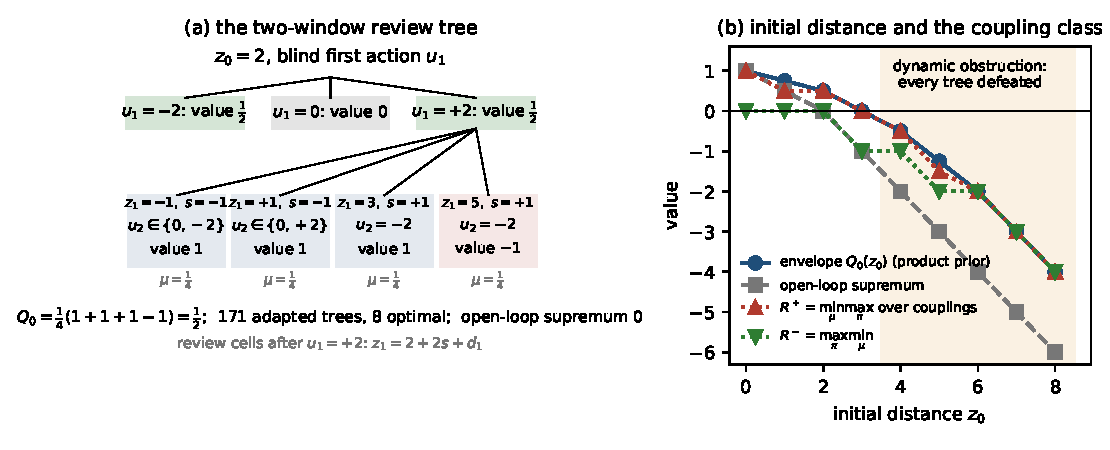
\includegraphics[width=\textwidth]{fig3_review.pdf}
\caption{The two-window instance (Theorem~\ref{thm:envelope}, Proposition~\ref{prop:robust}, Example~\ref{ex:sweep}). (a) The review tree at $z_0=2$: first-stage values, and the four review cells after $u_1=+2$ with their node values and optimal second actions. (b) Envelope $Q_0$, open-loop supremum and the robust values $R^\pm$ over the coupling class $\calM$ as functions of the initial distance $z_0$; the shaded region $z_0\ge4$ is the dynamically certified obstruction, where every adapted tree is defeated with positive probability.}
\label{fig:review}
\end{figure}

\subsection{Robust values over a class of couplings}

The product prior is one coupling of the one-step marginals; a robust reading lets an adversary choose the coupling. Let $\calM\subset\calP(\Omega)$ be a polytope of laws containing $\mu$ (in the instance: all laws on $\{\pm1\}^3$ with uniform coordinate marginals, a polytope of dimension $4$ with six vertices, whose barycentre is the product prior).

\begin{proposition}[robust envelope: weak duality and its closure]\label{prop:robust}
Let $\Pi$ be the finite set of adapted trees and define the lower and upper robust values
\begin{equation}\label{eq:robust}
R^-=\max_{\pi\in\Pi}\ \min_{\mu'\in\calM}\E_{\mu'}[G^\pi],\qquad R^+=\min_{\mu'\in\calM}\ \max_{\pi\in\Pi}\E_{\mu'}[G^\pi].
\end{equation}
Then (i) $R^-\le R^+\le Q_0(\mu)$ for every $\mu\in\calM$; (ii) $R^+=\max_{w\in\Delta(\Pi)}\min_{\mu'\in\calM}\sum_\pi w_\pi\E_{\mu'}[G^\pi]$: mixing over trees closes the gap, and a pair $(\mu^\ast,w^\ast)$ with $\max_\pi\E_{\mu^\ast}G^\pi=\min_{\mu'\in\calM}\sum_\pi w^\ast_\pi\E_{\mu'}G^\pi$ certifies $R^+$ exactly; (iii) $R^+<0$ iff some coupling $\mu^\ast\in\calM$ defeats every tree in expectation, in which case under $\mu^\ast$ every tree is defeated on a set of positive $\mu^\ast$-measure; the pair ($\mu^\ast$, the recursion \eqref{eq:N} under $\mu^\ast$) is a dynamic certificate of obstruction checkable by one backward induction; (iv) all four quantities $R^\pm$, $Q_0$, and the certifying pair are rational when the data are, being optimal values and vertices of linear programmes.
\end{proposition}

\begin{proof}
(i) is weak duality (for every $\pi$ and $\mu'$, $\min_{\mu''}\E_{\mu''}G^\pi\le\E_{\mu'}G^\pi\le\max_{\pi'}\E_{\mu'}G^{\pi'}$) and $\mu\in\calM$ with Theorem~\ref{thm:envelope}(i). (ii) The payoff $(\mu',w)\mapsto\sum_\pi w_\pi\E_{\mu'}G^\pi$ is bilinear on the product of two polytopes, so von Neumann's theorem \cite{vonNeumann1928} gives $\min_{\mu'}\max_w=\max_w\min_{\mu'}$, and $\max_w$ of a linear function over the simplex is attained at a vertex, i.e. $\min_{\mu'}\max_w=R^+$. (iii) The first statement is the definition; if $\E_{\mu^\ast}G^\pi<0$ then $\mu^\ast\{G^\pi<0\}>0$. (iv) The inner minima are linear programmes over $\calM$ and the outer problems are linear programmes in $(\mu',t)$ or $(w,t)$.
\end{proof}

\begin{example}[initial distance, couplings and a certified dynamic obstruction]\label{ex:sweep}
Table~\ref{tab:sweep} lists, for the two-window instance and $z_0=0,\dots,8$, the envelope $Q_0$ under the product prior, the open-loop supremum, and $R^\pm$ over the class $\calM$ of couplings with uniform coordinate marginals; every entry is exact and $R^+$ is certified by a pair $(\mu^\ast,w^\ast)$ as in Proposition~\ref{prop:robust}(ii).
\begin{enumerate}[leftmargin=1.6em,itemsep=1pt]
\item \emph{Value of the review.} $Q_0-\text{open-loop}=0,\tfr14,\tfr12,1,\tfr32,\tfr74,2,2,2$: the review is worth nothing at $z_0=0$ and two units of margin from $z_0=6$ on.
\item \emph{The worst coupling can be interior.} At $z_0=2$, $R^+=\tfr12=Q_0$ and the worst coupling is the product prior itself, while each of the six extreme couplings of $\calM$ gives the controller strictly more ($2,2,1,2,1,2$). At $z_0=1$ and $z_0=5$ a non-product coupling is strictly worse than the prior ($R^+=\tfr12<\tfr34$ and $R^+=-\tfr32<-\tfr54$); at $z_0=3$ the worst coupling is supported on four of the eight paths and ties with the prior.
\item \emph{Mixing closes the gap.} At $z_0=2$, $R^-=0<R^+=\tfr12$: no single tree guarantees more than $0$ against all couplings, but the uniform mixture of four trees guarantees $\tfr12$. From $z_0=6$ on, $R^-=R^+=Q_0$: one tree is optimal against every coupling.
\item \emph{Dynamic obstruction.} At $z_0=3$ the envelope is $0$ and every tree is defeated with positive probability although some have zero expected loss. At $z_0=4$ every one of the $171$ trees has negative expectation under the prior and is defeated with probability at least $\tfr38$; $R^+=-\tfr12=Q_0$, so the prior is itself a worst coupling and the pair (prior, recursion) is the dynamic certificate of Proposition~\ref{prop:robust}(iii). This is the review-tree counterpart of the static certificate: an explicit measure under which no adapted policy survives.
\item \emph{Coupling selection is real.} With identical one-step marginals and $G=d_1d_2$, the product coupling gives $0$, the comonotone coupling $1$ and their $\rho$-mixture $\rho$: the one-step marginals under-determine the envelope, which is why $\calM$ must be declared.
\end{enumerate}
\end{example}

\begin{table}[t]
\centering\small
\caption{Two-window instance: envelope, open-loop supremum and robust values against the initial distance (Example~\ref{ex:sweep}); all entries exact, $R^+$ certified on both sides.}
\label{tab:sweep}
\begin{tabular}{lccccccccc}
\toprule
$z_0$ & 0 & 1 & 2 & 3 & 4 & 5 & 6 & 7 & 8\\
\midrule
envelope $Q_0$ (product prior) & $1$ & $\tfr34$ & $\tfr12$ & $0$ & $-\tfr12$ & $-\tfr54$ & $-2$ & $-3$ & $-4$\\
open-loop supremum & $1$ & $\tfr12$ & $0$ & $-1$ & $-2$ & $-3$ & $-4$ & $-5$ & $-6$\\
$R^+=\min_{\mu'}\max_\pi$ & $1$ & $\tfr12$ & $\tfr12$ & $0$ & $-\tfr12$ & $-\tfr32$ & $-2$ & $-3$ & $-4$\\
$R^-=\max_\pi\min_{\mu'}$ & $0$ & $0$ & $0$ & $-1$ & $-1$ & $-2$ & $-2$ & $-3$ & $-4$\\
\bottomrule
\end{tabular}
\end{table}

\subsection{The integrated certificate}\label{sec:integrated}

The static certificate pools rows at one instant. For a finite-horizon trajectory problem with a finite set of branches (hidden modes) and an information schedule, the same pooling applies to the terminal constraint slack integrated along the trajectory, and yields a certificate against every policy adapted to the schedule.

\begin{proposition}[integrated certificate with adapted controls]\label{prop:integrated}
Let $L$ be a finite set of branches, $U$ a compact convex control set, $T>0$, and for each $\ell\in L$ let the terminal slack of a constraint be an affine functional of the control path,
\begin{equation}\label{eq:slack}
F_\ell(u_\ell)=\beta_\ell-\int_0^T k_\ell(\sigma)^\top u_\ell(\sigma)\dd\sigma,
\end{equation}
with integrable kernels $k_\ell$. Let $(\calP_\sigma)_{\sigma\in[0,T]}$ be a refining information schedule (partitions of $L$), and call a family $(u_\ell)_{\ell\in L}$ of measurable $U$-valued controls \emph{adapted} if $u_\ell(\sigma)=u_{\ell'}(\sigma)$ whenever $\ell,\ell'$ lie in the same cell of $\calP_\sigma$. Then for every $\lambda\in\Delta(L)$ and every adapted family,
\begin{equation}\label{eq:gammah}
\min_{\ell\in L}F_\ell(u_\ell)\ \le\ \Gamma_h(\lambda)\ :=\ \sum_\ell\lambda_\ell\beta_\ell+\int_0^T\ \sum_{C\in\calP_\sigma}h_U\Bigl(-\sum_{\ell\in C}\lambda_\ell k_\ell(\sigma)\Bigr)\dd\sigma .
\end{equation}
Hence $\Gamma_h(\lambda)<0$ certifies that every adapted policy violates some branch's constraint at $T$. On the three-branch instance of the companion paper \cite{Abaee2026cert}---a planar double integrator $\ddot p=u$ with $U$ the hexagon $\conv\{\pm n_\ell\}$, $n_1=(1,0)$, $n_{2,3}=(-\tfr35,\pm\tfr45)$, initial states $p_\ell(0)=\tfr{34}{25}n_\ell$, $\dot p_\ell(0)=n_\ell$, facets $n_\ell^\top p\le2$, the branch revealed at time $\tau$ and horizon $T=\tau+1$---the kernels are $k_\ell(\sigma)=(T-\sigma)n_\ell$, the margins $\beta_\ell=\tfr{16}{25}-T$, and $\lambda=(\tfr38,\tfr5{16},\tfr5{16})$ gives
\begin{equation}\label{eq:gamma3}
\Gamma_h(\tau)=\tfrac{7}{50}-\tau ,
\end{equation}
so the review is obstructed for every $\tau>\tfr7{50}$; the threshold is sharp by the policy of the companion paper, and $\Gamma_h(\tau)=-\Gamma(\tau)$ in the companion's sign convention, where $\Gamma(\tau)=\tau-\tfr7{50}$ is the value of a minimisation programme.
\end{proposition}

\begin{proof}
$\min_\ell F_\ell\le\sum_\ell\lambda_\ell F_\ell=\sum_\ell\lambda_\ell\beta_\ell-\int_0^T\sum_{C\in\calP_\sigma}\Bigl(\sum_{\ell\in C}\lambda_\ell k_\ell(\sigma)\Bigr)^{\!\top}u_C(\sigma)\dd\sigma$, where $u_C(\sigma)$ is the common control of the cell $C$; and $-g^\top u\le h_U(-g)$ for $u\in U$. For the instance, $\sum_\ell\lambda_\ell n_\ell=0$ kills the integrand on the blind window $[0,\tau)$, where the schedule has the single cell $L$; after $\tau$ the cells are singletons and $h_U(-n_\ell)=1$ because $-n_\ell$ is a vertex of the hexagon and $\|n_\ell\|=1$; $\int_\tau^T(T-\sigma)\dd\sigma=\tfr12$; and $\tfr{16}{25}-(\tau+1)+\tfr12=\tfr7{50}-\tau$. The slack \eqref{eq:slack} is $2-n_\ell^\top p_\ell(T)$ with $n_\ell^\top p_\ell(T)=\tfr{34}{25}+T+\int_0^T(T-\sigma)n_\ell^\top u_\ell(\sigma)\dd\sigma$.
\end{proof}

Two features of \eqref{eq:gammah} matter beyond the instance. First, the support function is evaluated at the \emph{negative} pooled kernel; on the centrally symmetric hexagon the sign is immaterial, but on a translated control set the two conventions differ (check G1.3), and the certificate of an asymmetric actuator must use \eqref{eq:gammah} as written. Second, the identity reproduces the one-step theory: a schedule with a single instant and a single cell is Theorem~\ref{thm:dual}'s weak direction with $k_\ell$ the drift coefficients. The converse---that $\Gamma_h<0$ for some $\lambda$ whenever every adapted policy fails---is the finite-horizon bridge theorem of the companion paper \cite{Abaee2026cert}, proved there by a mesh-exact linear programme; it is not re-proved here.

\begin{figure}[t]
\centering
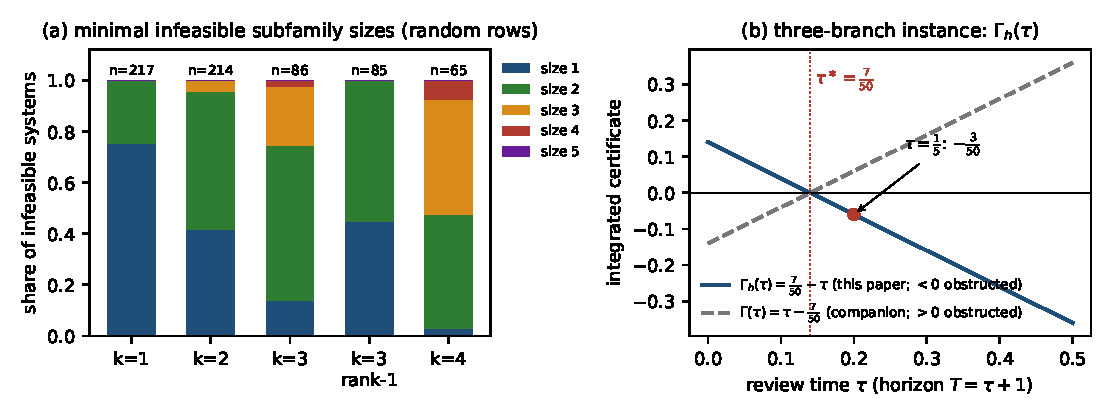
\includegraphics[width=\textwidth]{fig4_helly_gamma.pdf}
\caption{(a) Minimal infeasible subfamily sizes of random row systems with $m=k+3$ rows on $[-1,1]^k$ (Remark~\ref{rem:random}; $n$ is the number of infeasible systems among the draws). The size $k+1$ of Theorem~\ref{thm:helly} is attained but rare; with rank-one coefficients in $k=3$ the size never exceeds $2$. (b) The integrated certificate of the three-branch instance, $\Gamma_h(\tau)=\tfr7{50}-\tau$ (Proposition~\ref{prop:integrated}), against the companion's $\Gamma(\tau)=\tau-\tfr7{50}$; both cross zero at $\tau^\ast=\tfr7{50}$.}
\label{fig:helly}
\end{figure}
\section{Verification record and scope}\label{sec:verification}

\paragraph{Exact script.} Every value, witness, count and tabulated entry of the paper is regenerated from the definitions by \path{paper04_minimax_dual_certificates_v20_verification.py} with the exact module \texttt{p04\_core.py} (standard-library rational arithmetic; SciPy's HiGHS is used only to \emph{propose} dual weights and maximisers, which are then rationalised and verified exactly, with exact fall-backs when SciPy is absent). The script runs $66$ checks in under two minutes: the lower values and certificates of the static instances and the tight family up to $k=4$ (S1--S2); the random Helly-size study with its float screen confirmed exactly (S3); the benchmark caps from the model equations, the margin law, the uniqueness of the certificate, the Farkas pair and the demand-floor law on rational grids (B1--B4); the two-patch kernels (T1); the two-window envelope, the enumeration of all $171$ trees with tower and martingale identities, the committed-prefix identity, the posterior-only counterexample, the initial-distance sweep with both robust values certified on both sides, the extreme couplings by two independent enumerations and the dynamic obstruction (D1--D3); the inherited instances A ($2^{14}$ trees), B ($243$ trees), the refinement pair ($1024$ and $4096$ trees) and the matching instance (D4); the integrated certificate with the sign-convention control (G1); the Lean scope list (L1); and, after compilation, the binding of the theorem numbers quoted in captions and of the supplement's cross-reference table to the compiled \texttt{.aux} file (TXT). The figure script recomputes every plotted number from the same module. The supplementary material lists all checks with their outputs.

\paragraph{Lean footprint.} The Lean~4 module \cite{deMoura2021} \texttt{Minimax\_Dual.lean} (prelude-only, over an ordered-field interface, no \texttt{sorry}) contains $22$ theorem declarations, of which $13$ are arithmetic helpers and $9$ are the named footprints: \texttt{dual\_certificate\_sound} (a measure with strictly negative pooled row on every action proves that no common safe action exists, for any finite-mass measure and any action type); \texttt{parity\_common\_safe\_empty} and \texttt{parity\_no\_measure\_certifies} (both halves of Proposition~\ref{prop:nonconvex}(iii)); \texttt{two\_row\_average}, \texttt{ψsingle\_sum}, \texttt{singleton\_uniform}, \texttt{singleton\_every\_measure}, \texttt{singleton\_worst\_witnesses} (the singleton recoveries: on a one-state atom every measure certifies iff the worst row is negative); and \texttt{benchmark\_obstruction} ($c_1+c_2<2\le u_1+u_2$ implies $\tfr12((c_1-u_1)+(c_2-u_2))<0$, the algebra of Proposition~\ref{prop:benchmark}(iii)). Not formalised: the Sion converse (Theorem~\ref{thm:dual}), Helly sparsity (Theorem~\ref{thm:helly}), the polyhedral recovery in general (Theorem~\ref{thm:polyhedral}), and the whole dynamic layer; these are proved on paper and exercised by the script.

\paragraph{Claimed and not claimed.}
\begin{itemize}[leftmargin=1.4em,itemsep=1pt]
\item \emph{Proved in general:} Theorems~\ref{thm:dual}, \ref{thm:helly}, \ref{thm:polyhedral}; Propositions~\ref{prop:nonconvex}, \ref{prop:taxonomy}, \ref{prop:robust}, \ref{prop:integrated} (inequality \eqref{eq:gammah}); Theorem~\ref{thm:envelope} and Corollary~\ref{cor:prefix} for finite review problems.
\item \emph{Proved on the instance, exactly:} the benchmark laws (Propositions~\ref{prop:benchmark}, \ref{prop:floor}), the two-window sweep and robust values, the three-branch threshold \eqref{eq:gamma3}, the two-patch counts.
\item \emph{Observed, not proved:} the frequencies of Remark~\ref{rem:random}, which depend on the sampling law.
\item \emph{Not claimed:} that the first-order test is sufficient for viability along the benchmark band; a converse of \eqref{eq:gammah} (the companion's bridge theorem is cited, not re-proved); completeness of certificates for non-convex action sets beyond convexification; any statement about continuous-time or infinite-horizon review envelopes, which are formulated as open problems in Section~\ref{sec:related}.
\end{itemize}
\section{Related work, discussion and open problems}\label{sec:related}

\paragraph{Viability and set invariance.} The first-order safe-action set is the contingent-cone condition of viability theory \cite{Aubin1991,Aubin2011}, whose exactness under constraint qualifications goes back to Nagumo \cite{Nagumo1942}; the controlled-invariance literature for linear systems with polyhedral constraints \cite{Blanchini1999} computes the same objects by linear programming. Partial observation enters viability theory through guaranteed kernels and set-valued observers \cite{Cardaliaguet2007}, which give sufficient conditions; the common-action obstruction is the necessary first-order condition they must respect, and Theorem~\ref{thm:dual} is its certificate. Barrier certificates \cite{PrajnaJadbabaie2004} and control barrier functions \cite{Ames2017} certify safety; the measure certificate certifies the opposite, that no control satisfies the barrier condition on an atom, and it is sparse. Hamilton--Jacobi reachability \cite{Mitchell2005} computes the full-information value; the gap between $V^+$ and $V^-$ in Remark~\ref{rem:isaacs} is what partial information removes.

\paragraph{Minimax, Farkas and semi-infinite duality.} The use of Sion's theorem to turn an existence question into a measure is classical in semi-infinite programming \cite{HettichKortanek1993,AndersonNash1987} and in robust optimisation \cite{BenTalNemirovski1999,BenTal2009}; the specialisation to affine rows and a compact convex action set gives the exactness, and Helly's theorem gives the support bound that Carath\'eodory alone would miss by one. The scenario approach \cite{CalafioreCampi2006,CampiGaratti2008} finds the same number $k+1$ as the number of support constraints of a random convex programme; the connection is that both count the constraints a Helly argument needs. The adjustability question of Wei and Zhang \cite{WeiZhang2024}---when do adaptive decisions improve on static ones in a two-stage robust linear programme---is the open-loop gap of Table~\ref{tab:sweep} for linear data.

\paragraph{Dynamic games and information design.} The envelope of Section~\ref{sec:dynamic} is the finite partially observed dynamic programme \cite{Astrom1965,BertsekasShreve1978} written on review trees; upper and lower values are those of Isaacs \cite{Isaacs1965} and Ba\c{s}ar and Olsder \cite{BasarOlsder1999}. The robust value over couplings is a problem of information design \cite{BergemannMorris2019} with the coupling as the designer's instrument; the observation that the worst coupling can be interior to the class (Example~\ref{ex:sweep}) is the dynamic analogue of the mixing in Theorem~\ref{thm:dual}. The companion papers supply the continuous bridge \cite{Abaee2026cert}, the probabilistic layer \cite{Abaee2026prob} and the set-valued calculus \cite{Abaee2026calc} that the present dual serves.

\paragraph{What the certificate is for.} The reader who needs only the verdict can solve the primal linear programme. The certificate is for three other uses: it is \emph{portable} (a few rows and one support-function evaluation, checkable by a proof assistant); it is \emph{diagnostic} (support and facet multipliers run the three tests of Section~\ref{sec:taxonomy}); and it is \emph{prescriptive} with prices (the benchmark's five units of stock per unit of demand floor, the three-branch instance's $\tfr7{50}$). The same three uses carry over to the dynamic layer: the pair (coupling, recursion) is a portable dynamic certificate, the sweep is a diagnostic, and the open-loop gap prices the review.

\paragraph{Open problems.}
\begin{openproblem}[continuous review envelopes]\label{op:continuous}
Formulate the envelope of Definition~\ref{def:tree} for continuous state and observation spaces with action-dependent observations and prove the tree-supremum identity under measurable selection, including the case where the controller's actions determine which cells are observed; the finite theory here should be its exact restriction.
\end{openproblem}
\begin{openproblem}[robust envelopes beyond polytopes]\label{op:robust}
Extend Proposition~\ref{prop:robust} to classes of couplings defined by moment constraints or Wasserstein balls, and characterise when the worst coupling is extreme rather than interior.
\end{openproblem}
\begin{openproblem}[exact integrated duality]\label{op:integrated}
Identify conditions under which the inequality \eqref{eq:gammah} is tight for every refining schedule without passing through a mesh programme, i.e. a Sion-type theorem on the space of adapted controls with action-independent schedules; the three-branch instance shows the bound is tight at the threshold.
\end{openproblem}
\begin{openproblem}[non-convex residuals]\label{op:nonconvex}
For finite action sets, find a certificate notion for the residual obstruction (obstructed on $U$, not on $\conv U$) that is sparser than the full combinatorial check and sound; the parity instance is the smallest test.
\end{openproblem}
\section*{Declarations}
\paragraph{Funding.} None.
\paragraph{Conflicts of interest.} None.
\paragraph{Data availability.} No external data were used; all instance data are rational constants listed in the text and in the supplementary material.
\paragraph{Code availability.} The exact module \texttt{p04\_core.py}, the verification script with its output, the figure script and the Lean module are publicly available in the repository \url{https://github.com/MIKEAA2020/general-sustainability}; they reproduce every value, witness, count, figure and tabulated entry reported here.
\paragraph{AI declaration.} Large language models assisted with drafting, code review and iterative revision. The author reviewed and edited all outputs, re-ran all computations, and takes responsibility for the final work.

\begin{thebibliography}{99}\footnotesize

\bibitem{Abaee2026calc} Abaee, A., 2026. An obstruction calculus for viability under incomplete observation. Figshare preprint, version 2. \url{https://doi.org/10.6084/m9.figshare.33716593.v2}.

\bibitem{Abaee2026cert} Abaee, A., 2026. Finite certificates of nonviability under incomplete observation: a continuous-to-finite bridge with exact witnesses. Companion manuscript, \url{https://github.com/MIKEAA2020/general-sustainability}.

\bibitem{Abaee2026prob} Abaee, A., 2026. Probabilistic sufficiency under partial observation: belief-state safety values, survivable-set antichains, and the exact price of late information. Companion manuscript, \url{https://github.com/MIKEAA2020/general-sustainability}.

\bibitem{Ames2017} Ames, A.D., Xu, X., Grizzle, J.W., Tabuada, P., 2017. Control barrier function based quadratic programs for safety critical systems. \emph{IEEE Transactions on Automatic Control} 62(8), 3861--3876.

\bibitem{AndersonNash1987} Anderson, E.J., Nash, P., 1987. \emph{Linear Programming in Infinite-Dimensional Spaces}. Wiley, Chichester.

\bibitem{Astrom1965} \AA str\"om, K.J., 1965. Optimal control of Markov processes with incomplete state information. \emph{Journal of Mathematical Analysis and Applications} 10(1), 174--205.

\bibitem{Aubin1991} Aubin, J.-P., 1991. \emph{Viability Theory}. Birkh\"auser, Boston.

\bibitem{Aubin2011} Aubin, J.-P., Bayen, A.M., Saint-Pierre, P., 2011. \emph{Viability Theory: New Directions}, 2nd ed. Springer, Berlin.

\bibitem{BasarOlsder1999} Ba\c{s}ar, T., Olsder, G.J., 1999. \emph{Dynamic Noncooperative Game Theory}, 2nd ed. SIAM Classics in Applied Mathematics 23, Philadelphia.

\bibitem{BenTalNemirovski1999} Ben-Tal, A., Nemirovski, A., 1999. Robust solutions of uncertain linear programs. \emph{Operations Research Letters} 25(1), 1--13.

\bibitem{BenTal2009} Ben-Tal, A., El Ghaoui, L., Nemirovski, A., 2009. \emph{Robust Optimization}. Princeton University Press, Princeton.

\bibitem{BergemannMorris2019} Bergemann, D., Morris, S., 2019. Information design: a unified perspective. \emph{Journal of Economic Literature} 57(1), 44--95.

\bibitem{BertsekasShreve1978} Bertsekas, D.P., Shreve, S.E., 1978. \emph{Stochastic Optimal Control: The Discrete-Time Case}. Academic Press, New York.

\bibitem{Blanchini1999} Blanchini, F., 1999. Set invariance in control. \emph{Automatica} 35(11), 1747--1767.

\bibitem{CalafioreCampi2006} Calafiore, G.C., Campi, M.C., 2006. The scenario approach to robust control design. \emph{IEEE Transactions on Automatic Control} 51(5), 742--753.

\bibitem{CampiGaratti2008} Campi, M.C., Garatti, S., 2008. The exact feasibility of randomized solutions of uncertain convex programs. \emph{SIAM Journal on Optimization} 19(3), 1211--1230.

\bibitem{Cardaliaguet2007} Cardaliaguet, P., Quincampoix, M., Saint-Pierre, P., 2007. Differential games through viability theory: old and recent results. In: J{\o}rgensen, S., Quincampoix, M., Vincent, T.L. (Eds.), \emph{Advances in Dynamic Game Theory}, Annals of the International Society of Dynamic Games 9, Birkh\"auser, Boston, 3--35.

\bibitem{Chvatal1983} Chv\'atal, V., 1983. \emph{Linear Programming}. W.H. Freeman, New York.

\bibitem{deMoura2021} de Moura, L., Ullrich, S., 2021. The Lean 4 theorem prover and programming language. In: \emph{Automated Deduction -- CADE 28}, Lecture Notes in Computer Science 12699, Springer, 625--635.

\bibitem{Farkas1902} Farkas, J., 1902. Theorie der einfachen Ungleichungen. \emph{Journal f\"ur die reine und angewandte Mathematik} 124, 1--27.

\bibitem{Helly1923} Helly, E., 1923. \"Uber Mengen konvexer K\"orper mit gemeinschaftlichen Punkten. \emph{Jahresbericht der Deutschen Mathematiker-Vereinigung} 32, 175--176.

\bibitem{HettichKortanek1993} Hettich, R., Kortanek, K.O., 1993. Semi-infinite programming: theory, methods, and applications. \emph{SIAM Review} 35(3), 380--429.

\bibitem{Isaacs1965} Isaacs, R., 1965. \emph{Differential Games}. Wiley, New York.

\bibitem{Mitchell2005} Mitchell, I.M., Bayen, A.M., Tomlin, C.J., 2005. A time-dependent Hamilton--Jacobi formulation of reachable sets for continuous dynamic games. \emph{IEEE Transactions on Automatic Control} 50(7), 947--957.

\bibitem{Nagumo1942} Nagumo, M., 1942. \"Uber die Lage der Integralkurven gew\"ohnlicher Differentialgleichungen. \emph{Proceedings of the Physico-Mathematical Society of Japan}, 3rd series, 24, 551--559.

\bibitem{PrajnaJadbabaie2004} Prajna, S., Jadbabaie, A., 2004. Safety verification of hybrid systems using barrier certificates. In: \emph{Hybrid Systems: Computation and Control (HSCC 2004)}, Lecture Notes in Computer Science 2993, Springer, 477--492.

\bibitem{Rockafellar1970} Rockafellar, R.T., 1970. \emph{Convex Analysis}. Princeton University Press, Princeton.

\bibitem{Sion1958} Sion, M., 1958. On general minimax theorems. \emph{Pacific Journal of Mathematics} 8(1), 171--176.

\bibitem{vonNeumann1928} von Neumann, J., 1928. Zur Theorie der Gesellschaftsspiele. \emph{Mathematische Annalen} 100, 295--320.

\bibitem{WeiZhang2024} Wei, N., Zhang, P., 2024. Adjustability in robust linear optimization. \emph{Mathematical Programming} 208, 581--628.

\end{thebibliography}

\end{document}
